% !Mode:: "TeX:UTF-8"	% read in as utf8 file.

\chapter{Failure theories}
In materials science, the strength of a material is its ability to withstand an applied load without failure or plastic deformation. The field of strength of materials deals with forces and deformations that result from their acting on a material. A load applied to a mechanical member will induce internal forces within the member called stresses when those forces are expressed on a unit basis. The stresses acting on the material cause deformation of the material in various manners. Deformation of the material is called strain when those deformations too are placed on a unit basis. The applied loads may be axial (tensile or compressive), or rotational (strength shear). The stresses and strains that develop within a mechanical member must be calculated in order to assess the load capacity of that member. This requires a complete description of the geometry of the member, its constraints, the loads applied to the member and the properties of the material of which the member is composed. With a complete description of the loading and the geometry of the member, the state of stress and of state of strain at any point within the member can be calculated. Once the state of stress and strain within the member is known, the strength (load carrying capacity) of that member, its deformations (stiffness qualities), and its stability (ability to maintain its original configuration) can be calculated. The calculated stresses may then be compared to some measure of the strength of the member such as its material yield or ultimate strength. The calculated deflection of the member may be compared to a deflection criteria that is based on the member's use. The calculated buckling load of the member may be compared to the applied load. The calculated stiffness and mass distribution of the member may be used to calculate the member's dynamic response and then compared to the acoustic environment in which it will be used. \\

\begin{figure}[h!]
	\centering
	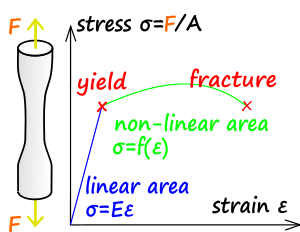
\includegraphics[width=0.5\linewidth]{figure/tension_test}
	\caption{Basic static response of a specimen under tension}
	\label{fig:tensiontest}
\end{figure}

Material strength refers to the point on the engineering stress–strain curve (yield stress) beyond which the material experiences deformations that will not be completely reversed upon removal of the loading and as a result the member will have a permanent deflection. The ultimate strength refers to the point on the engineering stress–strain curve corresponding to the stress that produces fracture.

\section{Strength terms}
Uniaxial stress is expressed by

\begin{equation}\label{eq: uniaxial stress}
\sigma ={\frac{F}{A}}
\end{equation} 

where $ F $ is the $ force [N] $ acting on an area $ A [m^2] $. The area can be the undeformed area or the deformed area, depending on whether engineering stress or true stress is of interest.\\

Mechanical properties of materials include the yield strength, tensile strength, fatigue strength, crack resistance, and other characteristics. \\

\begin{figure}[h!]
\centering
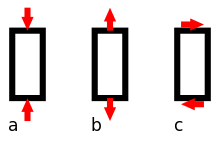
\includegraphics[width=0.3\linewidth]{figure/Compressive_tensile_shear_loading}
\caption{A material being loaded in a) compression, b) tension, c) shear}
\label{fig:compressivetensileshearloading}
\end{figure}

\begin{itemize}
	\item Yield strength is the lowest stress that produces a permanent deformation in a material. In some materials, like aluminium alloys, the point of yielding is difficult to identify, thus it is usually defined as the stress required to cause \SI{0.2}{\percent} plastic strain. This is called a \SI{0.2}{\percent} proof stress.
	\item Compressive strength is a limit state of compressive stress that leads to failure in a material in the manner of ductile failure (infinite theoretical yield) or brittle failure (rupture as the result of crack propagation, or sliding along a weak plane - see shear strength).
	\item Tensile strength or ultimate tensile strength is a limit state of tensile stress that leads to tensile failure in the manner of ductile failure (yield as the first stage of that failure, some hardening in the second stage and breakage after a possible "neck" formation) or brittle failure (sudden breaking in two or more pieces at a low stress state). Tensile strength can be quoted as either true stress or engineering stress, but engineering stress is the most commonly used.
	\item Fatigue strength is a measure of the strength of a material or a component under cyclic loading,[7] and is usually more difficult to assess than the static strength measures. Fatigue strength is quoted as stress amplitude or stress range ( $ \Delta\sigma= \sigma_\mathrm{max} - \sigma_\mathrm{min} $), usually at zero mean stress, along with the number of cycles to failure under that condition of stress.
	\item Impact strength, is the capability of the material to withstand a suddenly applied load and is expressed in terms of energy. Often measured with the Izod impact strength test or Charpy impact test, both of which measure the impact energy required to fracture a sample. Volume, modulus of elasticity, distribution of forces, and yield strength affect the impact strength of a material. In order for a material or object to have a high impact strength the stresses must be distributed evenly throughout the object. It also must have a large volume with a low modulus of elasticity and a high material yield strength.
\end{itemize}

\section{Failure theories}
There are four failure theories: maximum shear stress theory, maximum normal stress theory, maximum strain energy theory, and maximum distortion energy theory. Out of these four theories of failure, the maximum normal stress theory is only applicable for brittle materials, and the remaining three theories are applicable for ductile materials. Of the latter three, the distortion energy theory provides most accurate results in majority of the stress conditions. The strain energy theory needs the value of Poisson’s ratio of the part material, which is often not readily available. The maximum shear stress theory is conservative. For simple unidirectional normal stresses all theories are equivalent, which means all theories will give the same result. \\

\begin{itemize}
	\item Maximum Shear stress Theory- This theory postulates that failure will occur if the magnitude of the maximum shear stress in the part exceeds the shear strength of the material determined from uniaxial testing.
	
	\item Maximum normal stress theory - This theory postulates that failure will occur if the maximum normal stress in the part exceeds the ultimate tensile stress of the material as determined from uniaxial testing. This theory deals with brittle materials only. The maximum tensile stress should be less than or equal to ultimate tensile stress divided by factor of safety. The magnitude of the maximum compressive stress should be less than ultimate compressive stress divided by factor of safety.
	
	\item Maximum strain energy theory - This theory postulates that failure will occur when the strain energy per unit volume due to the applied stresses in a part equals the strain energy per unit volume at the yield point in uniaxial testing.
	
	\item Maximum distortion energy theory - This theory is also known as shear energy theory or von Mises-Hencky theory. This theory postulates that failure will occur when the distortion energy per unit volume due to the applied stresses in a part equals the distortion energy per unit volume at the yield point in uniaxial testing. The total elastic energy due to strain can be divided into two parts: one part causes change in volume, and the other part causes change in shape. Distortion energy is the amount of energy that is needed to change the shape.
\end{itemize}

For ductile materials there are two commonly used strength theories - the Maximum Shear Stress (MSS) or Tresca theory and the von Mises or Distortion Energy theory.

\subsection{Maximum Shear Stress:}
This states that failure occurs when the maximum shear stress in the component
being designed equals the maximum shear stress in a uniaxial tensile test at the
yield stress:\\

This gives $ \tau_{\max} = \frac{S_y}{2n} $ or $ | \sigma_1 – \sigma_2 | = \frac{S_y}{n} $ or $ | \sigma_2 – \sigma_3 | = \frac{S_y}{n} $ or $ | \sigma_3 – \sigma_1 | = \frac{S_y}{n} $ \\

whichever of the last three leads to the safest result. The latter usually involves $ \sigma_3 $ being zero, i.e. plane stress, and both $ \sigma_1 $ and $ \sigma_2 $ having the same sign. Note that the yield strength is reduced by the factor of safety $ n $.

\subsection{von Mises or Distortion Energy Theory:}
\subsubsection{distortion energy}
For ductile metals and alloys, according to the Maximum Shear Stress failure theory (aka “Tresca”) the only factor that affects dislocation slip is the maximum shear stress in the material. This is really a 1-dimensional explanation; a single parameter (maximum shear stress) is the only thing that causes yielding. However, the Tresca theory does work well in a 3-dimensional world. None the less, a slight improvement upon Tresca’s theory is warranted. Yielding (dislocation slip) is somewhat better explained (i.e. it is better supported by empirical data) by considering strain energy. \\

If we apply a load to a material it will deform. The units of energy are force*distance, so when a load is applied and the material deforms, we are putting energy into the material. This energy introduced into the material due to the loading is referred to as “strain energy.” We prefer to normalize strain energy by unit volume, and when we do so, this is referred to as strain energy density. The area under a stress-strain curve is the energy per unit volume (stress*strain has
units of force per area such as $ N/mm^2 $, which is the same as energy per unit volume $ N-mm/mm^3 $. We will be assuming linear elastic material only. Most metals and alloys are linear elastic prior to the onset of plastic deformation, so this is a valid assumption. \\

The strain energy is composed of two distinct forms – volume changes and distortion (angular change). Normal strains cause a change in volume, shear strain cause distortions. The total stain energy is the sum of distortion energy and volume energy:

\begin{equation}\label{key}
U_\mathrm{total} = U_\mathrm{distortion} + U_\mathrm{volume}
\end{equation}

Where
$ U_\mathrm{total}= $ total strain energy,\\
$ U_{distortioin}= $ strain energy due to distortioni,\\
$ U_\mathrm{volume}= $ strain energy due to volume change (aka hydrostatic strain energy)\\

We will develop equations for total strain energy $ (U_\mathrm{total}) $ and volume energy $ (U_\mathrm{volume}) $, anddetermine the distortion energy (which is really what we are interested in) from: \\

\begin{equation}\label{key}
U_\mathrm{distortion} = U_\mathrm{total} - U_\mathrm{volume}
\end{equation}

For general (3D) loading, the total strain energy is given in terms of principal stresses and strains:

\begin{equation}\label{eq: total strain energy}
U_\mathrm{total} = \frac{1}{2} \left( \epsilon_1 \sigma_1 + \epsilon_2 \sigma_2 + \epsilon_3 \sigma_3 \right)
\end{equation}

Using Hooke’s law $ \epsilon_1 = [\sigma_1 – \nu (\sigma_2 + \sigma_3 )] / E $ , etc. the total strain energy equation \ref{eq: total strain energy} can be written in terms of stress only:

\begin{equation}\label{eq: total strain energy in stress}
U_\mathrm{total} = \frac{1}{2} E \left( \sigma_1^2 + \sigma_2^2 + \sigma_3^2 -2 \nu \left(\sigma_2 \sigma_3 + \sigma_1 \sigma_3 + \sigma_1 \sigma_2 \right) \right)
\end{equation}

Remember that hydrostatic stress causes volume change and that it is invariant (hydrostatic stress is a scalar – it is not directionally dependent – therefore it does not vary depending upon axis orientation). “Invariant” means “does not vary.” The hydrostatic stress can be determined from the average magnitudes of the three principal stresses:

\begin{equation}\label{eq: hydrostatic energy}
\sigma_\mathrm{hydrostatic} = \sigma_\mathrm{ave} = \left(\sigma_1 + \sigma_2 + \sigma_3 \right) / 3
\end{equation}

$ \sigma_\mathrm{hydrostatic} $ is the stress condition that causes volume change. It is invariant. For a moment, let’s consider it alone. Let’s consider a loading condition that was purely hydrostatic with magnitude of shydrostatic as calculated in equation \ref{eq: hydrostatic energy}. If the only stress in this material is $ \sigma_\mathrm{hydrostatic} $ then for this special loading condition the 3 principal stresses would be equal to $ \sigma_\mathrm{hydrostatic} (\sigma_1 = \sigma_2 = \sigma_3 = \sigma_\mathrm{hydrostatic} ) $. Equation \ref{eq: total strain energy in stress} would become:

\begin{equation}\label{eq: purely hydrostatic energy}
	U = \frac{1-2\nu}{6E} \left( \sigma_\mathrm{hyd}^2 + \sigma_\mathrm{hyd}^2 + \sigma_\mathrm{hyd}^2 + 2\left(\sigma_\mathrm{hyd}^2\sigma_\mathrm{hyd}^2+\sigma_\mathrm{hyd}^2\sigma_\mathrm{hyd}^2+\sigma_\mathrm{hyd}^2\sigma_\mathrm{hyd}^2\right)\right)
\end{equation}

For purely hydrostatic loading condition that we assumed in equation \ref{eq: purely hydrostatic energy}, there is no distortion energy $ (U_\mathrm{distortion} = 0) $ so $ U_\mathrm{total} = U_\mathrm{volume} $. But what about our part which may have distortion energy? Regardless of the existence of distortion energy or not, equation \ref{eq: purely hydrostatic energy} – being based on the invariant hydrostatic stress – is the energy due to volume change, $ U_\mathrm{volume} $:

\begin{equation}\label{eq: volume energy in hydro}
	U = \frac{3(-2\nu)}{2E}\sigma_\mathrm{hyd}^2
\end{equation}

Substituting equation \ref{eq: hydrostatic energy} into \ref{eq: volume energy in hydro} gives:

\begin{equation}\label{eq: volume energy in stress}
U_\mathrm{volume} = \frac{1-2\nu}{6E} \left(\sigma_1^2 + \sigma_2^2 + \sigma_3^2 +2\sigma_2\sigma_3 + 2\sigma_1\sigma_3 + 2\sigma_1\sigma_2 \right)
\end{equation}

To determine the strain energy due to distortion only (not volume change) we subtract equation \ref{eq: volume energy in stress} from equation \ref{eq: total strain energy in stress}:

\begin{equation}\label{eq: distortion energy in stress}
\begin{split}
U_\mathrm{distortion} &= U_\mathrm{total} - U_\mathrm{volume} \\
&= \frac{1}{2E} \left(\sigma_1^2+\sigma_2^2 + \sigma_3^2 - 2\nu\left(\sigma_2\sigma_3 + \sigma_1\sigma_3 +\sigma_1\sigma_2 \right)\right) - \frac{1-2\nu}{6E} \left(\sigma_1^2+\sigma_2^2 + \sigma_3^2 + 2\sigma_2\sigma_3 + 2\sigma_1\sigma_3 +2\sigma_1\sigma_2 \right) \\
&=\frac{1+\nu}{3E}\frac{(\sigma_1-\sigma_2)^2+(\sigma_2-\sigma_3)^2+(\sigma_3-\sigma_1)^2}{2}
\end{split}
\end{equation}

Remember, the Maximum Shear Stress theory works pretty well in predicting
yielding of ductile metals and alloys, but we are trying to improve upon it a bit. Why does Maximum Shear Stress theory work well? Because indeed it is shear stress that causes dislocation slip (aka plastic deformation). What sort of strain do shear stresses produce? They produce shear strains --- in other words, distortion. What is the equation for maximum shear stress? It is: $ \tau_{max} = (\sigma_1 - \sigma_3) / 2 $. It is the difference between principal stress divided by 2. What do we see in equation \ref{eq: distortion energy in stress}? The differences between all principal stress divided by 2. Equation \ref{eq: distortion energy in stress} combines the maximum shear stress in each of the 3 principal planes into a single equation. It should not be surprising that “distortion strain energy” is related to maximum shear stress. Shear stress cause shear strain, which is distortion. \\

The Distortion Energy failure theory (which we will discuss next) is a bit more mathematically sophisticated than the Maximum Shear Stress failure theory, but is really very similar. Rather than considering only the maximum shear stress at a point, it combines the maximum shear stress at a point in the 3 principal planes. These two theories give very similar results, but Distortion Energy does match empirical data better. 

\subsubsection{distortion energy failure theory}
For uniaxial tensile loading (as is used to create a stress-strain curve), $ \sigma_2 = \sigma_3 = 0 $, and at the onset of yielding, $ F/A = \sigma_1 = S_\mathrm{ys} $ (at onset of yielding).

\begin{figure}[h!]
\centering
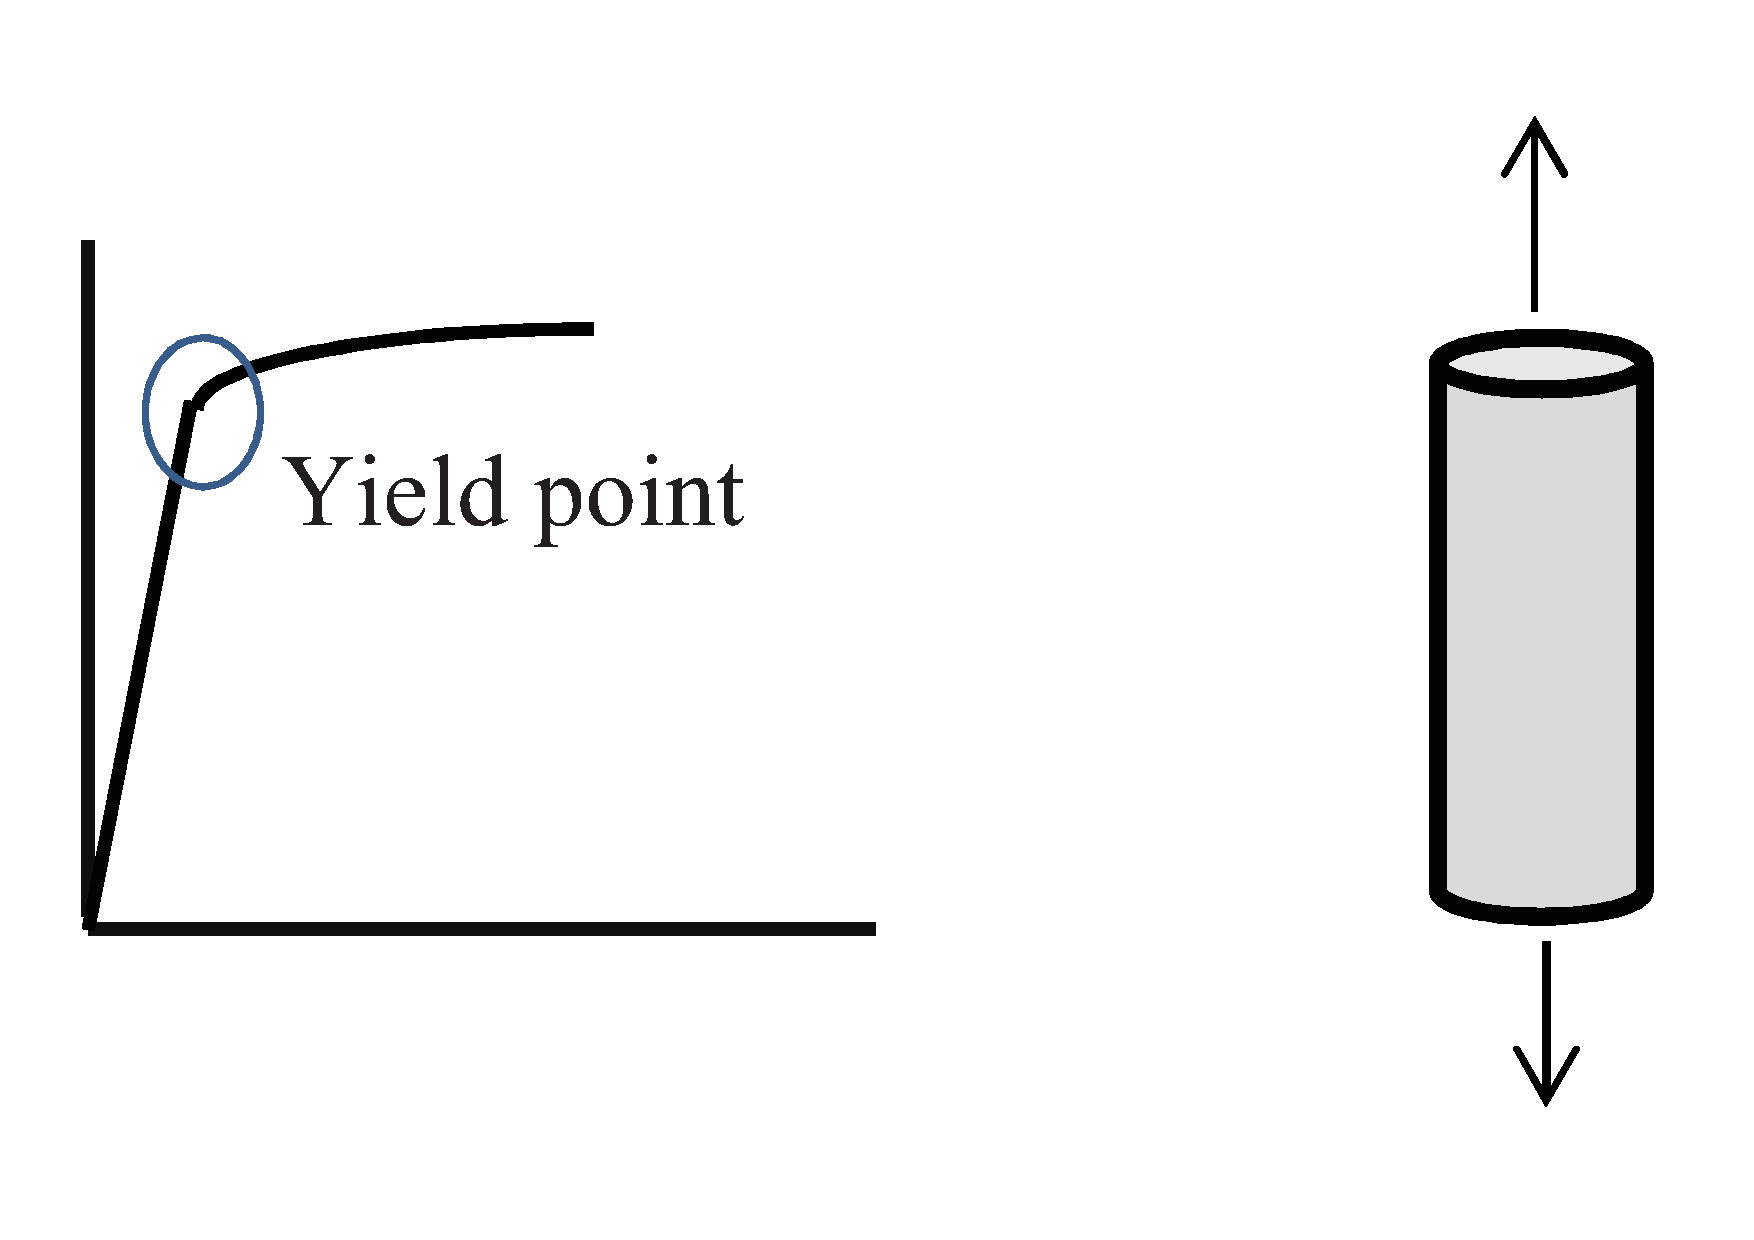
\includegraphics[width=0.5\linewidth]{figure/uniaxial_test_yield}
\caption{yield point in uniaxial test}
\label{fig:uniaxialtestyield}
\end{figure}

Therefore, for uniaxial loading at the onset of yielding (the stress shown on the stress-strain curve that we call “yield strength”) we substituting $ S_\mathrm{ys} $ for $ \sigma_1 $ and $ \sigma_2 = \sigma_3 = 0 $ into equation \ref{eq: distortion energy in stress}

\begin{equation}\label{eq: distortion energy in yield strength}
U_\mathrm{distortion} = \frac{1+\nu}{3E} S_\mathrm{ys}^2
\end{equation}

The Distortion Energy Theory states that when the distortion energy in a material equals or exceeds the distortion energy present at the onset of yielding in uniaxial loading tensile test for that material, the part will experience plastic deformation (i.e. it will yield):

\begin{equation}\label{eq: yield condition}
U_{distortion, part} \leq U_{distortion, uniaxial test} yielding occurs
\end{equation}

Equating the distortion energy in general 3-dimensional stress condition (equation \ref{eq: distortion energy in stress}) and distortion energy in simple uniaxial loading (equation \ref{eq: distortion energy in yield strength}); from equations \ref{eq: distortion energy in stress} and \ref{eq: distortion energy in yield strength} into equation \ref{eq: yield condition}:

\begin{equation}\label{key}
\begin{split}
\frac{1+\nu}{3E}\frac{(\sigma_1-\sigma_2)^2+(\sigma_2-\sigma_3)^2+(\sigma_3-\sigma_1)^2}{2} \leq \frac{1+\nu}{3E} S_\mathrm{ys}^2 \\
\sigma_\mathrm{eff} = \sqrt{\frac{(\sigma_1-\sigma_2)^2+(\sigma_2-\sigma_3)^2+(\sigma_3-\sigma_1)^2}{2}} \leq S_\mathrm{ys}
\end{split}
\end{equation}